\section*{FISICA 1 Fabrizio Cei \hfill 13|02|2024}
\subsection*{URTI E LEGGI DI CONSERVAZIONE}
Su un corpo che viene trascinato agiscono l'attrito STATICO (quando è fermo) e quello DINAMICO (quando si muove) che insieme costituiscono l'ATTRITO RADENTE.
Un corpo invece che rotola è soggetto all'ATTRITO VOLVENTE ($\ll$ dinamico).
Nel caso "ideale" si conservano:
\begin{itemize}
    \item $\bar{P}$ (quantità di moto) $\Rightarrow \Sigma \bar{F}_{ext} = 0, \bar{I}_{F_{ext}} = 0$
    \item $\bar{L}_0$ (momento angolare) $\Rightarrow \Sigma \bar{\tau}_{ext} = 0, \bar{I}_{\tau_{ext}} = 0$
    \item $K$ (energia cinetica) $\Rightarrow L_{diss} = 0$ ($U_i = U_f$ pk $\Delta t \to 0$)
\end{itemize}

\subsection*{Esempio 1}
Urto di un proiettile $m$ con una sbarretta $M, L$ non vincolata, appoggiata su un piano liscio. \textbf{Trattazione generale}.

\begin{figure}[H]
\centering
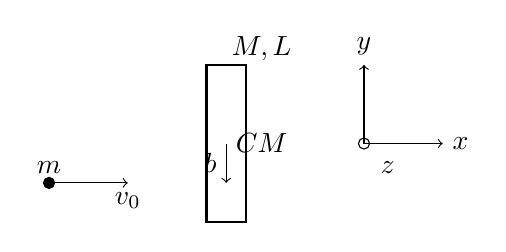
\begin{tikzpicture}
% sbarretta
\draw[thick] (2, -1) rectangle (2.5, 1);
\node at (2.7, 0) {$CM$};
\node at (2.7, 1.2) {$M, L$};
\draw[->] (2.25, 0) -- (2.25, -0.5) node[midway, left] {$b$};
% proiettile
\filldraw (0, -0.5) circle (2pt) node[above] {$m$};
\draw[->] (0, -0.5) -- (1, -0.5) node[below] {$v_0$};
% assi
\draw[->] (4, 0) -- (5, 0) node[right] {$x$};
\draw[->] (4, 0) -- (4, 1) node[above] {$y$};
\draw[->] (4, 0) circle (2pt);
\node at (4.3, -0.3) {$z$};
\end{tikzpicture}
\caption*{prima dell'urto}
\end{figure}

$b = \text{parametro d'impatto}$

- no forze esterne $\rightarrow$ SISTEMA ISOLATO: $\bar{P}$ costante
$$ \bar{P}_i = \bar{P}_{mi} + \bar{P}_{Mi} = m\bar{v}_0 + 0 = \bar{P}_f = \bar{P}_{mf} + \bar{P}_{Mf} = m\bar{v}' + M\bar{v}_{CM} $$
$$ \Rightarrow \bar{v}' = \bar{v}_0 - \frac{M}{m} \bar{v}_{CM} $$

- no momenti forze esterne $\rightarrow$ SISTEMA ISOLATO: $\bar{L}_0$ costante.
$O \equiv CM$ (comodo)
$$ \bar{L}_{CM}^i = \bar{b} \times \bar{p}_i = m \bar{b} \times \bar{v}_0 = \bar{L}_{CM}^f = \bar{b} \times \bar{P}_f = m \bar{b} \times \bar{v}' + \underbrace{I_{CM}}_{= ML^2/12} \cdot \bar{\omega} $$
$$ \Rightarrow \bar{\omega} = \frac{M}{I_{CM}} (\bar{b} \times \bar{v}_{CM}) $$
+ rotazione intorno a CM \\
+ traslazione del CM

L'urto avviene lungo $\hat{x}$:
$\bar{v}_{CM} = v_{CM} \hat{x} \Rightarrow \bar{\omega} = \omega \hat{z}$
$\bar{b} = -b \hat{y} \Rightarrow \bar{v}' = v' \hat{x}$
$$ v' = v_0 - \frac{M}{m} v_{CM} \; , \; \omega = \frac{12 M b v_{CM}}{M L^2} $$

- l'energia dipende dal tipo di urto
\begin{align*}
K_i &= K_{mi} = \frac{1}{2} m v_0^2 \\
K_f &= K_{mf} + K_{Mf} = \frac{1}{2} (m v'^2 + I_{CM} \omega^2 + M v_{CM}^2) \\
&= \frac{1}{2} m v_0^2 + \frac{1}{2} M \left(1 + \frac{M}{m} + \frac{12 b^2}{L^2}\right) v_{CM}^2 - M v_0 v_{CM}
\end{align*}
$$ \Rightarrow \Delta E = K_f - K_i = \frac{1}{2} M v_{CM}^2 \left( 1 + \frac{M}{m} + \frac{12 b^2}{L^2} - \frac{2 v_0}{v_{CM}} \right) $$

\subsubsection*{Caso 1: Urto totalmente anelastico ($\Delta E \neq 0$)}
\begin{figure}[H]
\centering
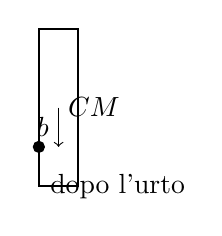
\begin{tikzpicture}
% sbarretta
\draw[thick] (2, -1) rectangle (2.5, 1);
\node at (2.7, 0) {$CM$};
% proiettile
\filldraw (2, -0.5) circle (2pt);
\draw[->] (2.25, 0) -- (2.25, -0.5) node[midway, left] {$b$};
\node at (3, -1) {dopo l'urto};
\end{tikzpicture}
\end{figure}

$$ v' = \omega b + v_{CM} = v_{CM} ( 1 + 12b^2/L^2 ) = v_0 - M v_{CM} / m $$
$$ \Rightarrow v_{CM} = \frac{v_0}{1 + \frac{M}{m} + \frac{12 b^2}{L^2}} $$
$$ \Rightarrow v' = \frac{v_0 (L^2 + 12b^2)}{12b^2 + \left(\frac{m+M}{m}\right) L^2} $$
$$ \Rightarrow \omega = \frac{m b v_0 \cdot 12}{(m+M)L^2 + 12 m b^2} $$
$$ \Rightarrow \Delta E = - \frac{m M}{2} \cdot \frac{(v_0 \cdot L)^2}{(m+M)L^2 + 12 m b^2} $$
